\section{Data Acquisition}
To download the data, we implemented the class \emph{ImageDownloader}. It automatically loads all fits files or only the ones of one run. When starting a run, the downloader will skip files already present on disk.
For all our experiments we used the images of run \emph{8162}.

\begin{listing}
    \begin{minted}[linenos]{python3}
def __align_image(self, reference: Union[PrimaryHDU, Cutout2D], other: PrimaryHDU, size: Optional[tuple] = None) -> tuple[Cutout2D, Cutout2D]:
    reference_wcs = (WCS(reference.header)
                        if not isinstance(reference, Cutout2D)
                        else reference.wcs)
    other_wcs = (WCS(other.header)
                    if not isinstance(other, Cutout2D)
                    else other.wcs)

    reference_coords = SkyCoord(
        ra=reference_wcs.wcs.crval[0]*u.deg,
        dec=reference_wcs.wcs.crval[1]*u.deg)
    other_coords = SkyCoord(
        ra=other_wcs.wcs.crval[0]*u.deg, dec=other_wcs.wcs.crval[1]*u.deg)

    cutout_1 = Cutout2D(reference.data, other_coords,
                        size=reference.data.shape if size is None else size, wcs=reference_wcs,
                        mode='partial', fill_value=0)
    cutout_2 = Cutout2D(other.data, reference_coords,
                        size=reference.data.shape if size is None else size, wcs=other_wcs,
                        mode='partial', fill_value=0)

    return cutout_1, cutout_2
        \end{minted}
    \label{alignementCode}
    \caption{The code we use to align an image pair}
\end{listing}

Alignement of the data is handled by the \emph{AlignementService}. In particular, the code seen in \Cref{alignementCode} handles the adjusting of two images. We then loop over all spectral bands and get the corresponding cutouts in reference to the first image. This results in a nicely aligned multichannel image.

The same \emph{AlignementService} also handles the label transcription from the fits format to the desired format. This is done because we need the WCS reference of the aligned cutouts to correctly calculate the pixel coordinates for each object.
We round the resulting coordinates to get one exact location in the image.

\begin{figure}
    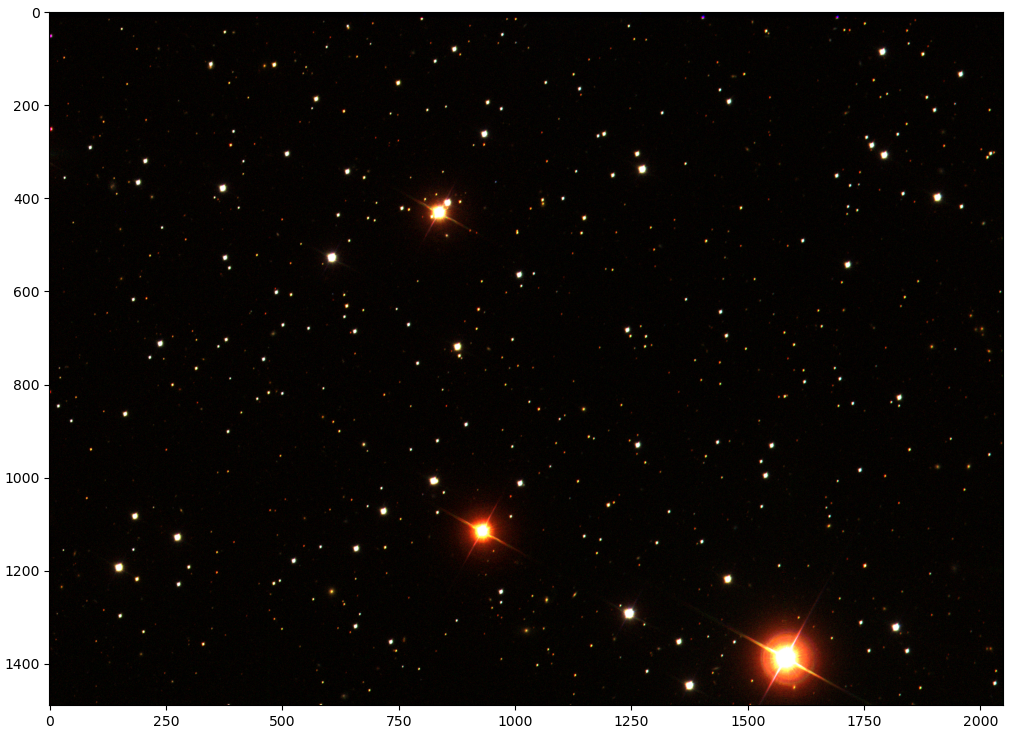
\includegraphics[width=\textwidth / 2]{aligned_validation_frame.png}
    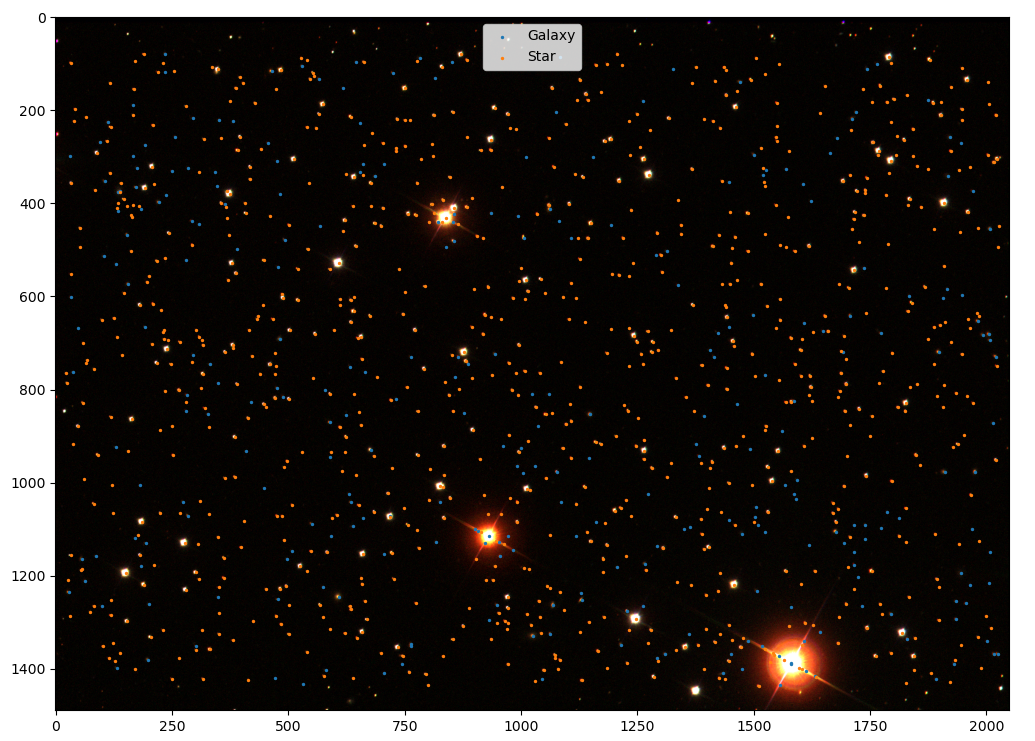
\includegraphics[width=\textwidth / 2]{aligned_validation_frame_with_labels.png}
    \caption{Aligned images with and without class markers}
    \label{alignedImages}
\end{figure}

In \Cref{alignedImages} the aligned spectral bands can be seen. In the second image, the dots indicate a labeled star or galaxy.

\section{Data Statistics}
\begin{figure}
    \begin{table}[H]
        \begin{tabularx}{\textwidth}{mmmmmm}
            \hline
                              & G          & R          & I          & U          & Z          \\
            \hline
            mean              & 0.01829018 & 0.06763462 & 0.03478437 & 0.00994593 & 0.09194765 \\
            \hline
            variance          & 0.6351227  & 1.1362617  & 0.8386613  & 0.7339489  & 3.5971174  \\
            \hline
            mean galaxies     & 0.3555972  & 0.66457057 & 0.41107112 & 0.5257245  & 1.7446687  \\
            \hline
            mean stars        & 1.7689778  & 2.3413954  & 1.8904239  & 0.7942855  & 4.4665427  \\
            \hline
            variance galaxies & 1.9958429  & 2.7264001  & 1.9724108  & 4.534722   & 11.216864  \\
            \hline
            variance stars    & 7.0836196  & 7.499741   & 6.6610627  & 6.519651   & 21.924402  \\
            \hline
        \end{tabularx}
    \end{table}
    \caption{Table containing the means and variances of our dataset}
    \label[type]{moments}
\end{figure}
We looked at the data quite extensively prior to classifying. Especially, we calculated mean and variance for the different color channels and with and without considering classes. The results can be seen in \Cref{moments}.
The variances of channel R and Z differ very much from the other ones. The large variance of the infrared channel Z could be related to redshift. Also the means of channel U and Z for galaxies and stars differ very much as well as all of the variances.


\begin{figure}
    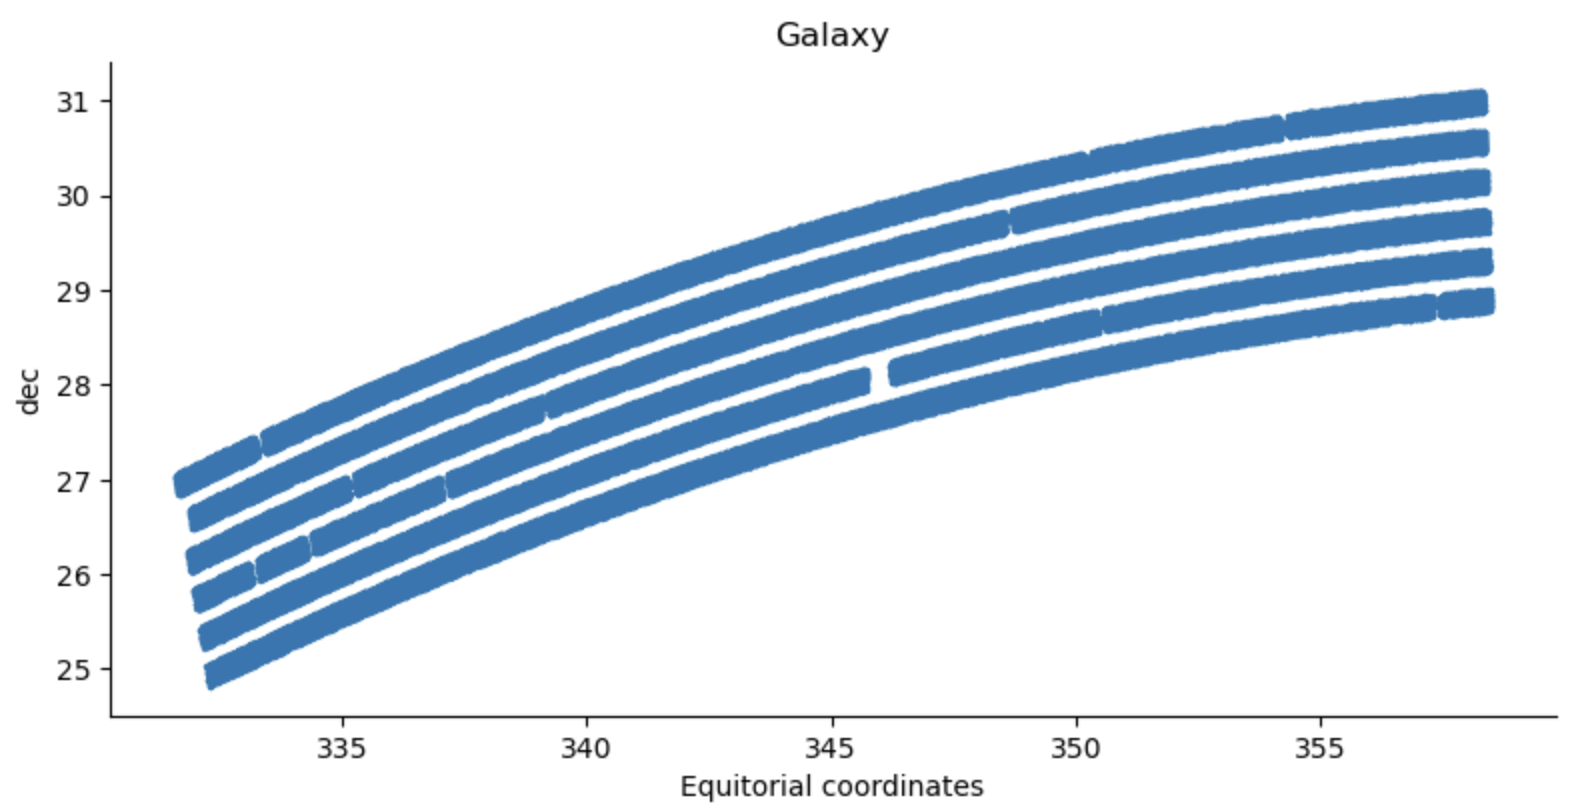
\includegraphics[width=\textwidth / 2]{Galaxies.png}
    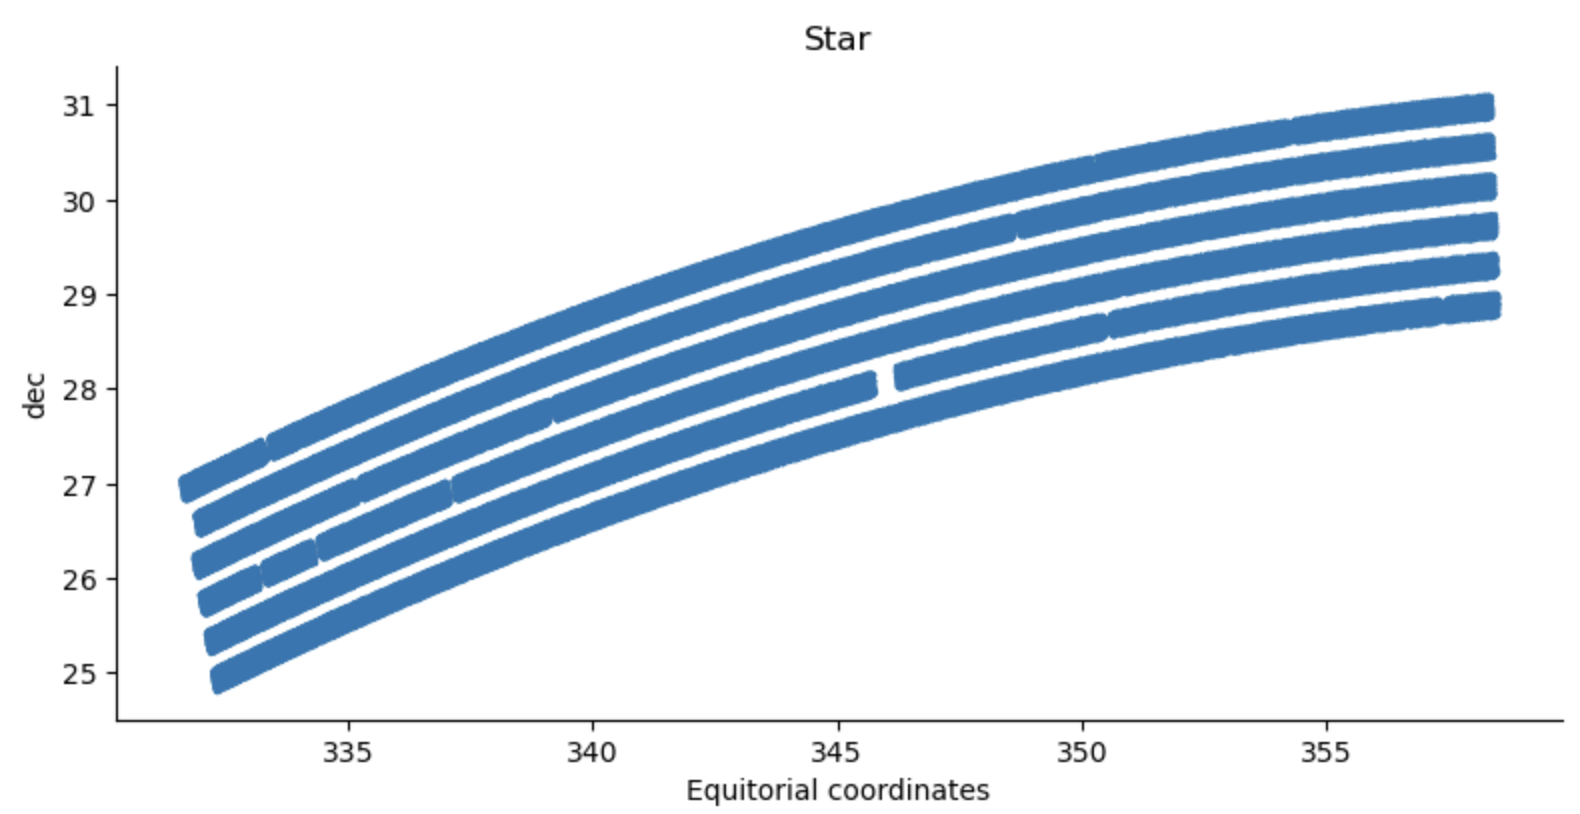
\includegraphics[width=\textwidth / 2]{Stars.png}
    \caption{Spatial distribution of the galaxies and starts in equatorial coordinates}
    \label{distributionPlots}
\end{figure}
Furthermore, we look at the spacial distribution of the classes. To do so, we plotted them in equatorial coordinates in \Cref{distributionPlots}. The blind spot in the middle the the proprietary evaluation field. The six distinct stripes are a result of the imaging technique. We do not see a difference in the spacial distribution of the two classes. The differences between the classes are minor.

Additionally to the spacial distribution, we calculated the number of samples per class. We got 287404 galaxies and  538043 stars in our whole dataset. These numbers are without the stated field in task 1.2.

\begin{figure}
    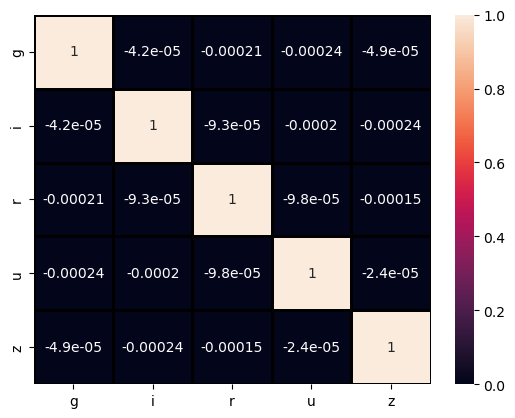
\includegraphics[width=\textwidth / 2]{color_correlation.png}
    \caption[short]{Correlation of the different color channels}
    \label{colorCorr}
\end{figure}
We also had a look at the correlation between the colors channels. These were very low. Some channels are not even correlated with themselves. All results can be seen in \Cref{colorCorr}.
